\section{Søvn Estimerings Model}
Med de valgte sensorer der bruges til søvnestimeringen fastlagt, grundet erfaringer fra andre kilder \textbf{REF HER}, består arbejdet i at konstruere en meningsfuld søvn estimerings model.

I \cref{sec:BES} nævnes en række features der udtrækkes fra deres sensor data i \citet{6563918}, men for at kunne gøre dette bør der ses på data fra sensorerne.
Dette resulterer i en bedre opfattelse af hvordan man kan bruge lyd og accelerationsdata, hvorefter en metode til at udtrække features fra disse data foreslås.
Til sidst resulterer dette i en samlet model der vægter features samlet fra lyd- og accelerations-data.

\subsection{Sensor Data}
Hovedideen bag brugen af accelerations og amplitude data kan ses i \cref{sec:BES}, men den dækker ikke alle problemscenarier der kan være involveret i brugen af disse data.

For at have en bedre indsigt i hvordan vi kan bruge accelerations og amplitude data blev disse plottet over en dag inklusiv søvn, hvor man holdt log for hvornår der blev sovet.
Dette resulterede i de plots der kan ses i \cref{fig:accplot} og \cref{fig:amplplot}.

\begin{figure}[h]
	\centering
	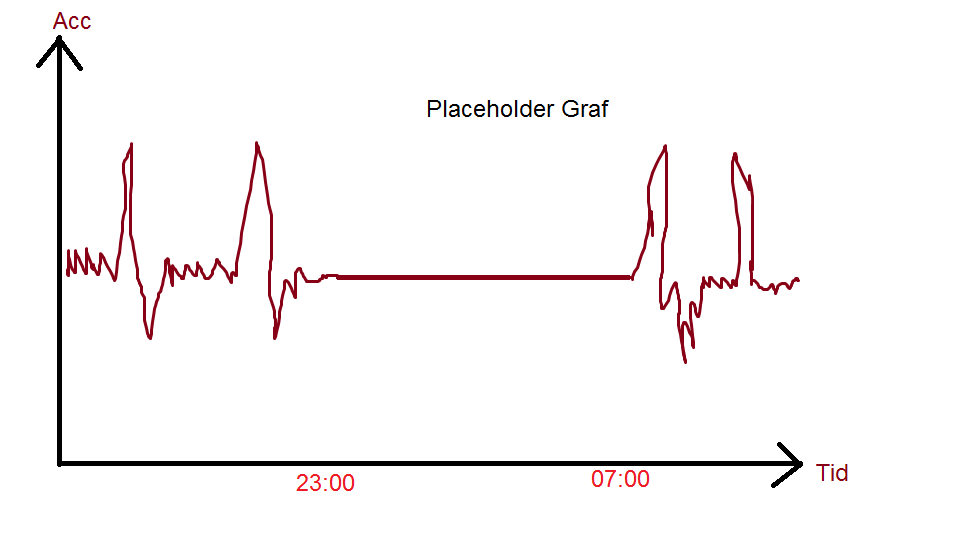
\includegraphics[scale=0.5]{acc-placeholder}
	\caption{Accelerationsplot, hvor der blev sovet fra 23:00 til 07:00 næste dag.}\label{fig:accplot}
\end{figure}

Ses der på accelerometer data i \cref{fig:accplot} indikerer det tydeligt når telefonen har været i bevægelse.
Dette skyldes at i sensorens natur er den god til at registrere bevægelse, da accelerationer er nødvendige for at ændringer i hastighed kan finde sted.
Der kan ses at antagelsen om at når man går med sin telefon i lommen er man vågen svarer fint til accelerations plottet.
Dog kan man ved stilstand ikke vide sig sikker på om det er forbi man sover, eller blot fordi man har lagt sin mobil fra sig.
Ved stilstand i en længere periode kan det forsøges at estimere sandsynligheden for at denne stilstand er grundet at man sover, men derudover kan andre sensor inputs hjælpe til at klargøre denne tvivl, der ikke er begrænset til at man skal have telefonen i lommen.
Et eksempel på en sådan kilde er mikrofonen vi kan bruge til at måle maksamplitude, således at man ikke indsamler personfølsomme oplysninger.

\begin{figure}[h]
	\centering
	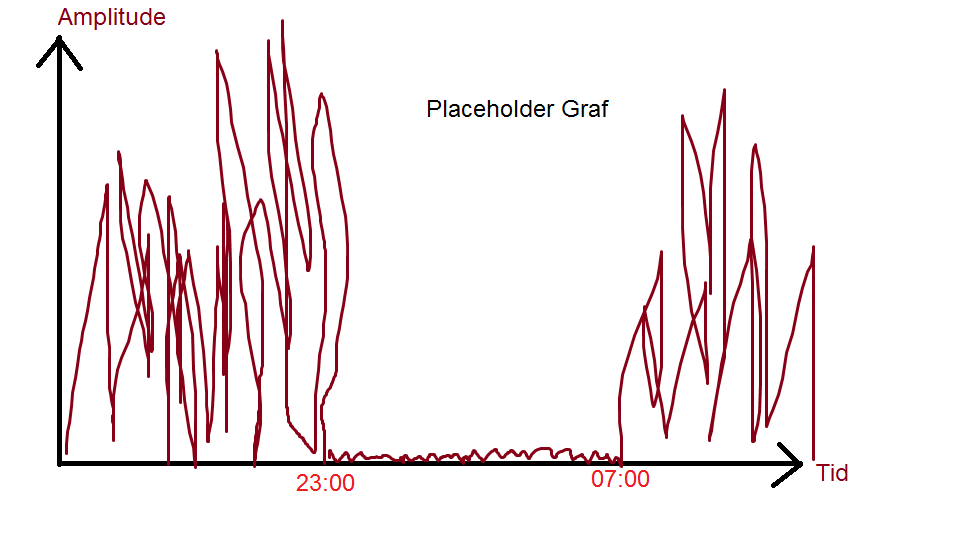
\includegraphics[scale=0.5]{ampl-placeholder}
	\caption{Amplitudeplot, hvor der blev sovet fra 23:00 til 07:00 næste dag.}\label{fig:amplplot}
\end{figure}

Idéen bag at bruge maksamplituden er at man larmer væsentligt mere når man er vågen end når man sover.
Dette passer fint med de loggede data plottet i \cref{fig:amplplot}.
Dog har denne antagelse også begrænsninger.
Eksempelvis kan det være at man er en stille person eller snorker meget.
Alligevel regner vi med at amplituden stadig kan bruges, da man så muligvis kunne finde et mønster når man snorker, og muligvis begiver sig hen i støjende områder når man er vågen. Derudover er det så et spørgsmål om hvor stor vægt man skal tillægge de enkelte sensorkilder og er noget der bør trænes til det enkelte individ for at opnå en model der passer til det enkelte individs personlighed.
Hvordan dette gøres bør overvejes, men som en start kan nogle fastsatte vægte bruges.

\subsection{Søvnestimerings model}
Ud fra observeret data etablerer vi nogle antagelser som vi går ud fra holder til fremtidigt data også.
Disse er at når man observerer en handling om det er acceleration eller amplitude, kan vi med stor sikkerhed sige at man ikke sover.
Modsat ved stilstand er sandsynligheden for at man sover afhængigt af længden af stilstand.
Dette får os til at lave en model der bygger på disse to antagelser.

Vi kan med andre ord sige følgende:
\begin{equation}
P(t,t_0) =
\begin{cases}
0	& t = t_0 \\
min(s(t-t_0),1) & \text{ellers}
\end{cases}
\end{equation}
hvor,
\begin{itemize}
	\item[$t$] Tiden for observeret data.
	\item[$t_0$] Sidste tid med bevægelse/lyd.
\end{itemize}
Hvis vi formulerer problemet på denne måde er det et spørgsmål om at ændre $t_0$ når der observeres et væsentligt udsving i ens data, der indikerer man er vågen.
Derudover vil $t-t_0$ så svare til længden af stilstand eksempelvis målt i timer.

Spørgsmålet går så på hvorledes $s(t-t_0)$ skal defineres.
Det skal være en funktion der repræsenterer hvor sikker man er på søvn ud fra længden af stilstand eksempelvis målt i timer.
En sådan funktion bør være lært ud fra ens empiri, så man kunne løse opgaven som et regressionsproblem.
Dette er et område der kan arbejdes videre med for at få en mere akkurat søvnestimeringsmetode og opfordres til at gøre med mere tid.

Dog for at få et udgangspunkt til diskussion af sådanne funktioner er der tre funktioner plottet i \cref{fig:trefunc}.
\begin{figure}[h]
	\centering
	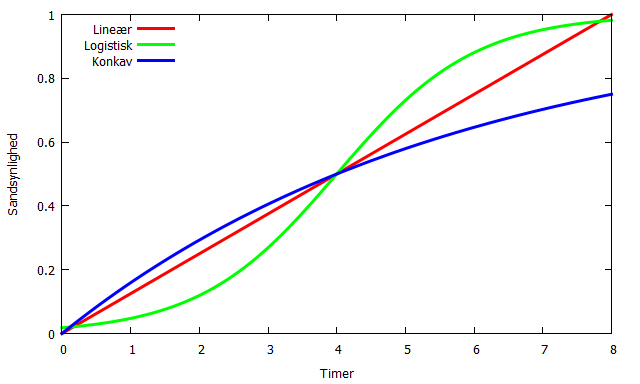
\includegraphics[scale=0.3]{graf-funktionseksempler}
	\caption{Tre funktioner til estimering af sandsynlighed for søvn}\label{fig:trefunc}
\end{figure}

\cref{fig:trefunc} viser tre forslag til funktioner for $s(t-t_0)$.
Disse er den røde lineære funktion, den blå konkave funktion og den grønne logistiske funktion.
Alle tre funktioner har til fælles at de er monotont voksende, hvilket passer med vores antagelse af jo længere der har været stilstand jo større sandsynlighed for at man sover.
Den lineære funktion bygger på antagelsen at sandsynligheden for at man sover er kongruent med stilstands længden, hvilket vi ikke ønsker da vi så tillægger for stor vægt til korte stilstandsperioder.
Af samme grund forkastes den konkave funktion også.

Til sidst har vi den logistiske funktion der fint beskriver hvordan at ved længere stilstandsperioden er der en forøget hældning i funktionen indtil vi nærmer os lange stilstandsperioder hvor ekstra tid ikke giver megen ekstra sandsynlighed for søvn men stadig lidt, dette kan ses da den logistiske funktion vi har plottet går asymptotisk mod 1, svarende til 100\% sikkerhed for søvn.
I realiteten kan vi aldrig være 100\% sikker på søvn ved lang stilstand, det kan være man har glemt mobilen hjemme mens man er på tur over en weekend, men hvis forudsætningen for at systemet fungerer er at man har mobilen i nærheden regnes den logistiske funktion som et godt redskab til et søvnestimat.

Definitionen af $s(t-t_0)$ hvor vi kalder $t-t_0$ for $t_{span}$ er dermed følgende:
\begin{equation}
	s(t_{span}) = \frac{L}{1+e^{k*(-t_{span} - t_{midpoint})}}
\end{equation} 
hvor,
\begin{itemize}
	\item[$t_{midpoint}$] er til hvilket stilstandslængde vi vil have sandsyngligheden for søvn til at være 50\%, dette kan eksempelvis være $4$ timer.
	\item[$k$] er stejlheden for kurven.
	\item[$L$] er kurvens maksimums værdi, hvilket for os eksempelvis kan være $1$ for 100\% sandsynlighed for søvn.
\end{itemize}

Der kan argumenteres for en lavere værdi for $L$ så man maks kan blive 90\% sikker, men er noget der bør overvejes med mere træningsdata.

Til sidst er der at orientere om hvordan vi afgør om der er stilstand, og dermed angiver en ny værdi for $t_0$, dette gøres i øjeblikket med en simpel metode der ser på de sidste 5 målinger og ser at afstanden mellem den observerede måling og de sidste fem målinger ikke overstiger et givet grænseværdi der estimeres ud fra træningsdataene, men i fremtiden bør der overvejes alternativer.

\subsection{Kombinering af modeller}
Det er tiltænkt at hver sensor kan have en tilknyttet søvnestimeringsmodel, hvilket i vores tilfælde er en søvnestimeringsmodel for accelerometer og mikrofon data.
Imidlertid kan det være en fordel at have en samlet model der kombinerer resultaterne fundet for de enkelte modeller.
En simpel metode at gøre dette på er v.h.a. et vægtet gennemsnit, hvilket er metode som \citet{6563918} også benytter.
Det vægtede gennemsnit kan udregnes på følgende måde:
\begin{equation}
	P_{kombineret}(t,t_0) = \sum_{i=1}^{n}{w_iP_i(t,t_0)}
\end{equation}
, hvor
\begin{itemize}
	\item[$P_{kombineret}(t,t_0)$] er den kombinerede sandsynlighed for søvn ved stilstand fra tiden $t_0$ til $t$.
	\item[$w_i$] er vægten som $P_i(t,t_0)$ skal tillægges.
	\item[$P_i(t,t_0)$] er sandsynligheden for søvn ved stilstand fra tiden $t_0$ til $t$ for sandlynlighedsmodellen $i$.
\end{itemize}
Dette er dog en forsimplet version af vores vægtede gennemsnit, i realiteten er der ikke data på samme tid eller i samme mængder for de enkelte søvnestimeringsmoduler.
Af samme grund ved mangel på en estimering til en given tid for et givent modul tages den seneste tid før denne.
Man kan forestille sig en lynlås hvor der skiftes mellem takkerne fra hver del, ligesom det gøres med estimeringerne for hvert modul.\als{SKAL HAVE EN BEDRE BESKRIVELSE}

